\documentclass{article}
\usepackage{amsmath}
\usepackage{forest}
\usepackage{tikz,pgf}
\usepackage{fancyhdr}
\pagestyle{fancy}
\fancyhf{}
\fancyhead[L]{CS3230 - Assignment 2}
\fancyhead[R]{Daniel Alfred (A0184588J)}
\fancyfoot[C]{\thepage}
\begin{document}
	\begin{enumerate}
		\item {
			\begin{align*}
				\Phi(T) &= |2 \cdot T.num - T.size|\\
				\text{let } x_i &= \text{the size of table deleted in step i}\\
				c_i &= 1 + x_i\\
				\hat{c}_i &= c_i + \Phi(D_i) - \Phi(D_{i-1})\\
				&= 1 + x_i + |2 \cdot T_i.num -T_i.size| - 
							  |2\cdot (T_i.num - 1) - (T_i.size - x_i)| \\
				&= 1 + x_i + 2 \cdot (T_i.num - (T_i.num - 1)) + 
									 (-T_i.size - (-T_i.size - x_i))\\
				&= 1 + x_i + 2 + -x_i\\
				&= 3
			\end{align*}
		}
		\pagebreak
		\item{
			\begin{align*}
				\text{Using accounting method:}&\\
				&\text{Enqueue}(x) = \$3\\
				&\text{Dequeue}(x) = \$0\\
				\text{Proof:}&\\
				\text{The money in the bank:}&\\
				&=\text{the number of element in stack1 +}\\
				&\text{number of element that haven't been popped (stack1 + stack2)}\\
				&= 2\cdot \text{element in stack1}+\text{element in stack2}\\
			\text{Enqueue}(x):&\\
				&\text{We need to pay \$3 for each operation}\\
				&\$1\text{ for insert}\\
				&\$1\text{ for later moving the number from stack 1 to stack 2}\\
				&\$1\text{ for later pop from stack 2}\\
				&\hat{c} = \$3 = \Theta(1)\\
			\text{Dequeue}(x):&\\
				&\text{We need to pay \$0 for each operation}\\
				&\$1\text{ from the bank for each element moved from stack1 to stack2}\\
				&\$1\text{ from the bank for popping from stack 2}\\
				&\hat{c} = \$0 = \Theta(0)\\
			\end{align*}	
		}
		\pagebreak
		\item{
			\begin{align*}
				\Phi'(D_i) &= \Phi(D_i) - \Phi(D_0)\\
				\text{Because of }& \Phi(D_i) \geq \Phi(D_0)\\
				\Phi'(D_i) &\geq 0\\
				\\
				\text{In $\Phi$:}&\\
				&\hat{c_i} = c_i + \Phi(D_i) - \Phi(D_{i - 1})\\
				\text{In $\Phi'$:}&\\
				&\hat{c_i} = c_i + \Phi'(D_i) - \Phi'(D_{i-1})\\
				&\hat{c_i} = c_i + \Phi(D_i) - \Phi(D_0) - (\Phi(D_{i-1} - \Phi(D-0))\\
				&\hat{c_i} = c_i + \Phi(D_i) - \Phi(D_{i-1})\\
			\end{align*}
		}
		\pagebreak
		\item{
			\begin{align*}
				&\text{Create 4 squares inside of a circle with $r$ radius}\\
				&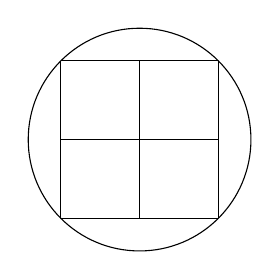
\begin{tikzpicture}
					\draw[step=1] (0, 0) grid (2, 2);
					\draw (1, 1) circle(sqrt(2););
				\end{tikzpicture}\\
				&\text{Each square have a side length of }\frac{r \sqrt{2}}{2}\\
				&\text{Create squares with that size inside of square size }l\cdot l\\
				&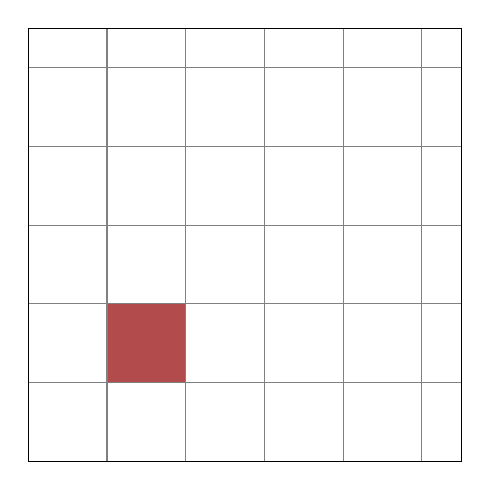
\begin{tikzpicture}
					\fill[red!40!gray] (1, 1) rectangle (2, 2);
					\draw[step=1, gray] (0, 0) grid (5.5, 5.5);
					\draw (0, 0) rectangle (5.5, 5.5);
				\end{tikzpicture}\\
				&\text{So we have $(\frac{l}{\frac{r \sqrt{2}}{2}})^2 = (\frac{2\cdot l}{r \sqrt{2}})^2 \approx \lceil\frac{2\cdot l^2}{r^2}\rceil$ smaller squares}\\
				&\text{If we choose any point inside the red square as the center point of the circle,}\\
				&\text{the whole red square is covered.}\\
				&\text{This will be a coupon collecting problem with $\lceil\frac{2\cdot l^2}{r^2}\rceil$ squares}\\
				&=O(\lceil\frac{2\cdot l^2}{r^2}\rceil)\\
				&=O(\lceil\frac{l^2}{r^2}\rceil)\\
			\end{align*}
		}
	\end{enumerate}     
\end{document}
